% !TEX root = ../Article.tex
\chapter{Smart Card Framework - Goals and Environment}
\label{ch:frameworkGoals}
As mentioned in section \ref{sec:goals} we want to create an Android framework allowing easy development of applications that utilizes smart card capabilities to enhance their security. The framework should implement basic communication protocols for different smart cards and basic out-of-the-box security functions. Both of these should be extendable so that developers can implement their own smart card based security. We want to achieve this not only for testing, but to be able to hand over a ready to use framework for any parties interested so that further development and testing may continue. In this chapter we will discuss the basis for the framework and the environment we will use for creating it.
%for easy communication between a mobile device and a smart card
The framework should lay the very foundation needed for using the mobile device and smart card in a secure fashion. The basic things we want to cover are:
\begin{itemize}
    \item Secure communication
    \item Key management
    \item Basic encryption
\end{itemize}
If we manage to create a framework covering these three points we believe that we have a great starting point for further testing and development.

\section{Design goals}
\label{sec:designAndroidGoals}
The framework should be functional and require little work to integrate into an application. Therefor the basic design goals for the framework will be:
\begin{itemize}
    \item Easy to use.
    \item Little to no understanding of Java Card and smart cards required.
    \item Extendable.
\end{itemize}

Even though most users of our framework will have a basic understanding of smart cards we believe that abstracting some central concepts will make the framework easier to use. One of the concepts we abstract is APDU. As a user/developer of the framework you can choose not to work with APDUs and use pre-implemented methods.

As we cannot possibly predict all types of uses for the framework we will also include a method for sending custom commands to the smart cards. This ensures that developers don't feel limited in how they can use the framework as well as catering to advanced users. More on the implemented methods in section \ref{sec:androidApp}.

Along with the Android framework we will also provide a simple Java Card applet that corresponds to the functionality we implement in the Android framework. This applet should follow the same principles as the Android framework, but will require some understanding of smart cards by the developer.

\section{Development tools and technology}
\label{sec:devAndTech}

\subsection{Smart card}
\label{sec:smartcardGemalto}
The first part of the complete framework is the application on the smart card. This part of the framework will perform the tasks that we can place on the smart card.

\paragraph{Java Card version}\mbox{}\\
%\subsection{Java Card version}
The cards we have support Java Card 2.2.2 and this is the version we will target. A natural question is ``Why don't we target Java Card 3 and above?''. Smart cards used for banking or handling other highly confidential data needs to be evaluated under the Common Criteria \cite[Ch.~26.3.2]{securityEngineering} standards. Potentially an application may handle confidential data and as a result we want smart cards with a Evaluation Assurance Level (EAL) 4 or above. Achieving EAL4 or above is an expensive and long process and relatively few products have this certification.


\begin{table}[h!]
\caption{Evaluation Assurance Level}
\label{tbl:EAL}
\centering

    \begin{tabular}{ | c | l |}
        \hline
        \thead{Level}
        & \thead{Description} \\ \hline

        1 & Functionally Tested \\ \hline
        2 & Structurally Tested \\ \hline
        3 & Methodically Tested and Checked \\ \hline
        4 & Methodically Designed, Tested and Reviewed \\ \hline
        5 & Semiformally Designed and Tested \\ \hline
        6 & Semiformally Verified Design and Tested \\ \hline
        7 & Formally Verified Design and Tested \\ \hline

    \end{tabular}
\end{table}

Table \ref{tbl:EAL} shows the difference between EAL levels. Comparing the EAL levels is a rather hard task (other than looking at their name and what they test) as there is no guarantee that what has been tested corresponds to the real world \cite[Ch.~26.3.3]{securityEngineering}.

When we decided on Java Card 2.2.2. we had to consider if we wanted a newer Java Card version with more functionality or if we wanted to comply with government directives (EAL requirements). The obvious choice was the latter as we have to comply with government directives.

The micro SD card we have access to are certified with EAL5, but only supports Java Card 2.2.2. \cite{gemaltoidgo8030}. This is also the case with the contact+contactless cards we have access to \cite{gemaltoidgo3010}. The Java Card operating system supports ``Java Card v2.2.2 (3.0.1 for the Elliptic Curves algorithms)'', which means that some of the cryptographic functionality of Java Card 3.0.1 is present. Refer to table \ref{tbl:algos} for available cryptographic algorithms.
\newpage
\begin{table}[h!]
\captionsetup{justification=centering,margin=1.5cm}
\caption{Available cryptographic algorithms in IDCore 3010 and IDCore 8030.}
\label{tbl:algos}
\centering

    \begin{tabular}{ | l | p{7cm} |}
        \hline
        \thead{Type}
        & \thead{Supported algorithms} \\ \hline

        Symmetric-key cryptography & 3DES (ECB, CBC), AES (128, 192, 256 bits) \\ \hline
        Public-key cryptography & RSA (up to 2048 (on-card generated), up to 4096 (off-card generated)) \\ \hline
        Hashing & SHA-1, SHA-224, SHA-256, SHA-384, SHA-512 \\ \hline
        Elliptic curves & ECC(up to p-521) \\ \hline

    \end{tabular}
\end{table}

\paragraph{Development environment}\mbox{}\\
%\subsection{Development environment}
In order to develop applications for the smart cards we will be using Eclipse 3.2 with Java development kit version 1.6.45. In order to develop smart card applications more easily we will use the Eclipse-JCDE plugin \cite{eclipseJCDE} which provides a virtual runtime environment along with build tools. Even though Eclipse 3.2 is severely outdated it provides the tools necessary to do the job.

\begin{figure}[h!]
  \caption{Screenshot of Eclipse Java Card tools.}
  \label{fig:eclipse}
  \centering
    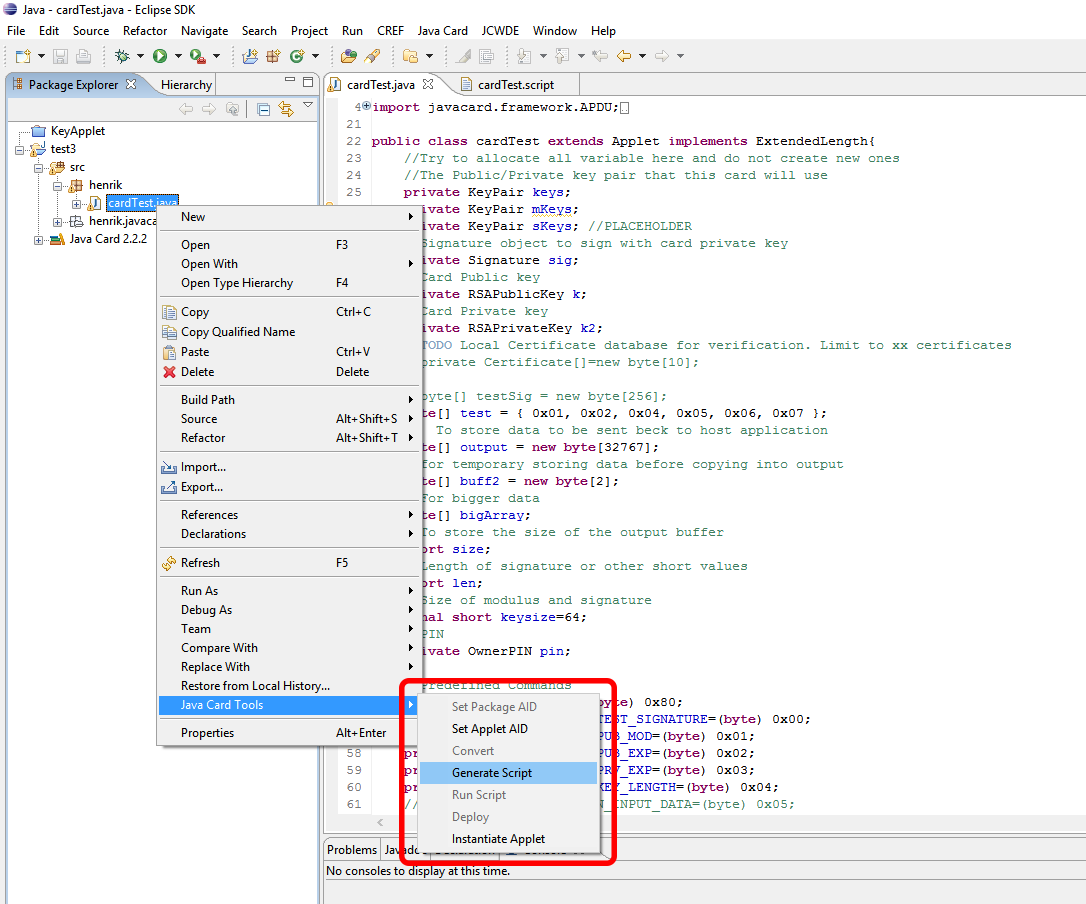
\includegraphics[width=0.95\textwidth]{images/eclipse.png}
\end{figure}

In figure \ref{fig:eclipse} we can see the tools for generating the deployable smart card application package (.cap file). The screenshot also shows how the editor looks like any other Eclipse version. Even though this version of Eclipse includes tools for sending and receiving APDUs to the application (testing), we have decided not to use these tools as they proved themselves to be unstable and not representative of real world use. This is mostly due to the fact that the application is deployed to an emulator and does not have \textit{any} hardware limitations of a physical smart card.
\newpage
\paragraph{Deployment}\mbox{}\\
We will be using GlobalPlatformPro (GP) \cite{globalplatform} to deploy and manage applets on the physical smart cards. GP is a command line tool and is compatible with our hybrid Gemalto card with reader as well as the micro SD card. In figure \ref{fig:deployFlow} we can see which part of the assembly line GP is responsible for. GP takes the generated .cap file and deploys it to the smart card via the card reader using the computer drivers.

\begin{figure}[h!]
  \caption{Deployment line using GlobalPlatformPro.}
  \label{fig:deployFlow}
  \centering
    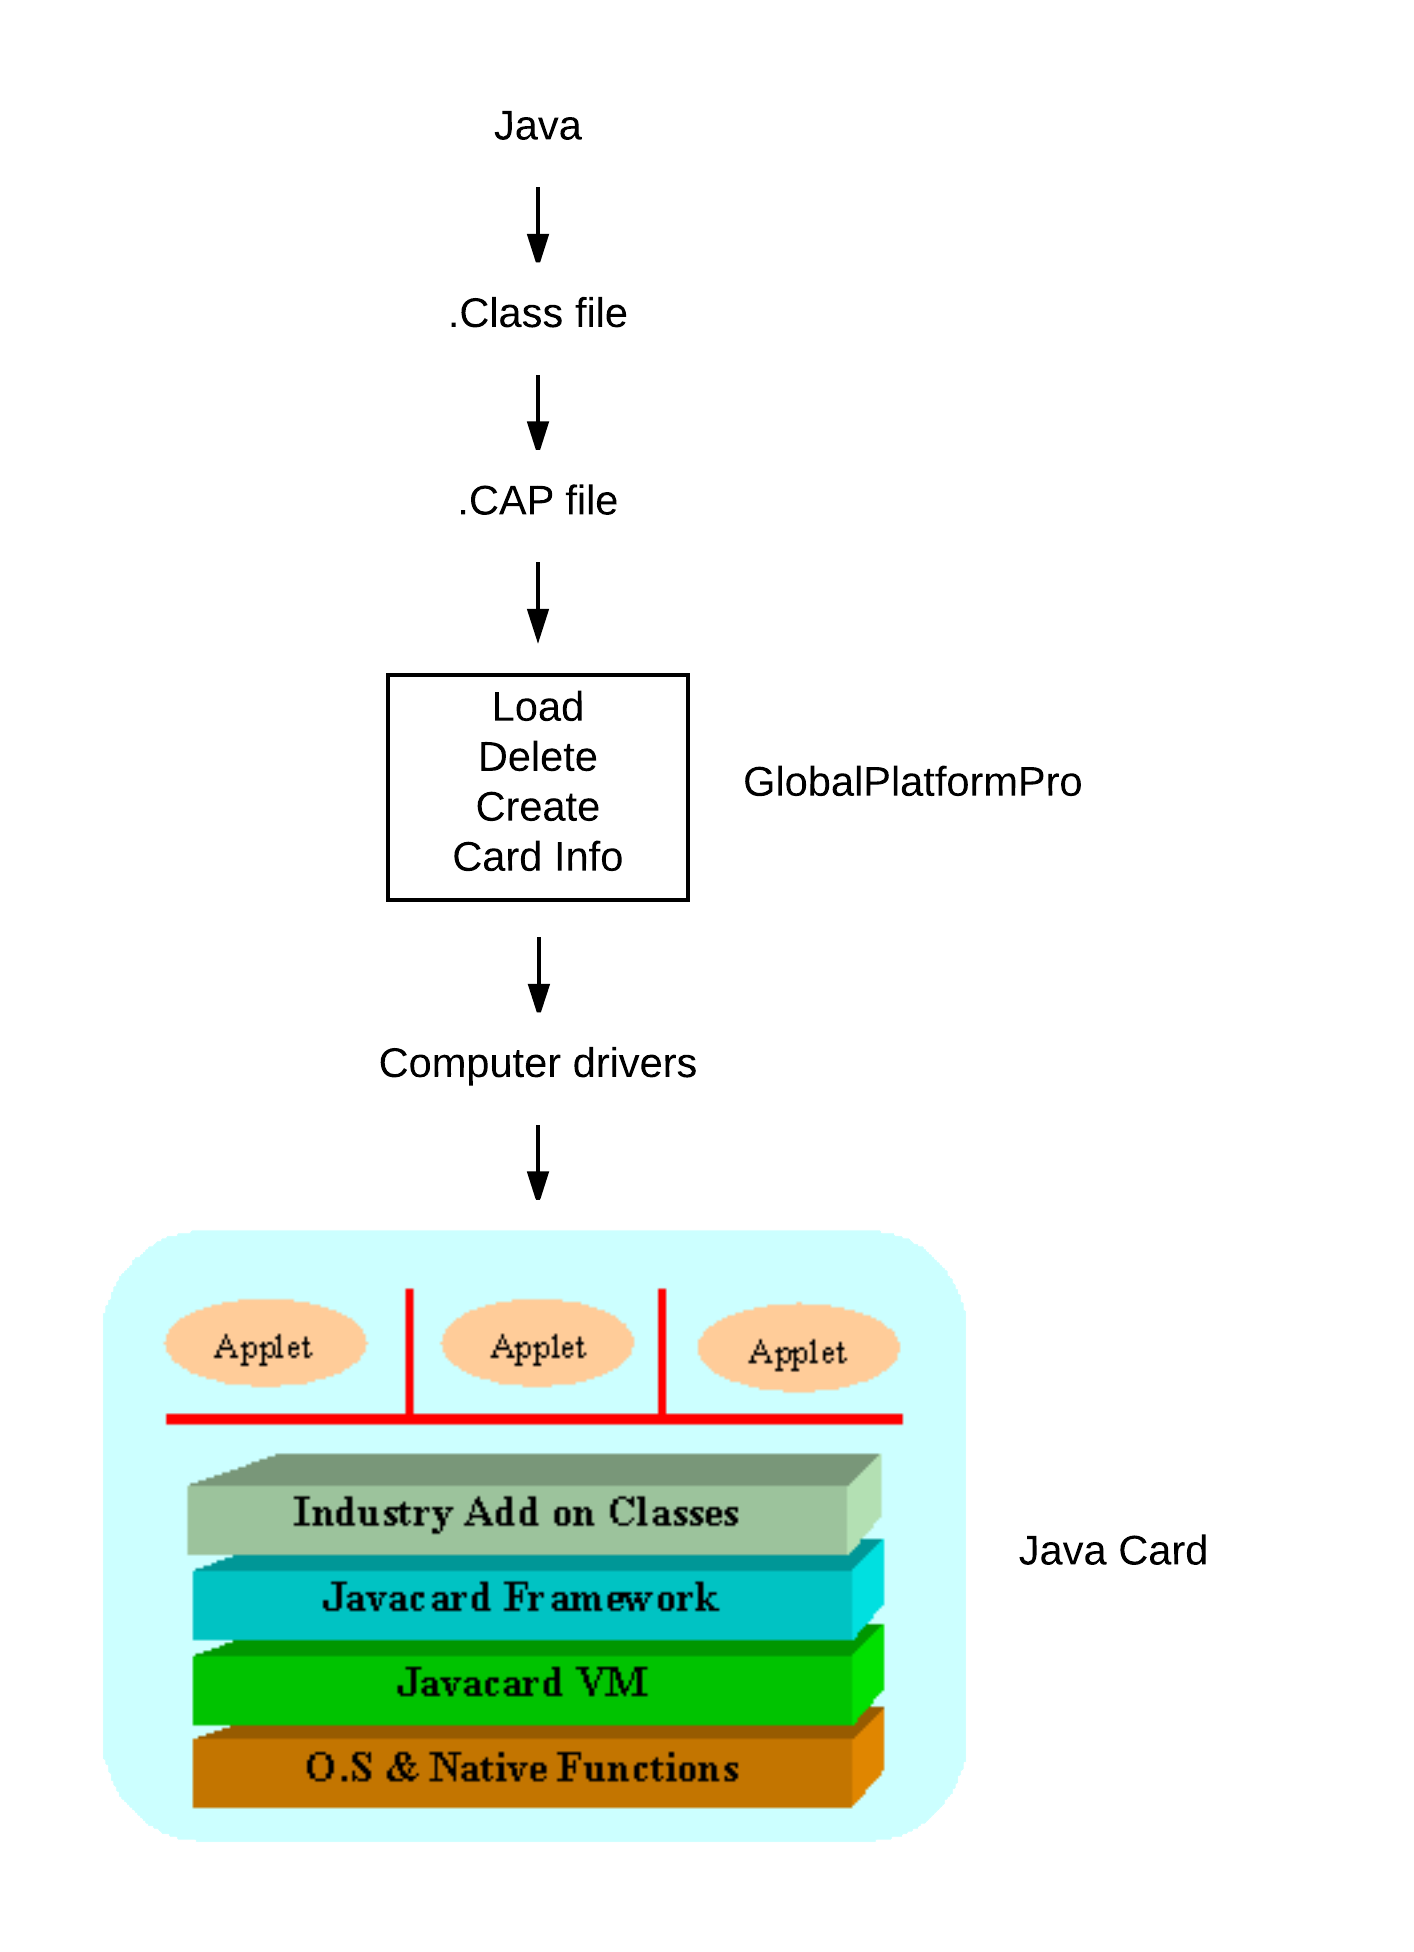
\includegraphics[width=0.65\textwidth]{images/deployFlow.png}
\end{figure}

There are three essential steps when deploying an application to a smart card:
\begin{itemize}
    \item Delete the smart card application along with the stored data.
    \item Delete the smart card package.
    \item Install the new smart card application.
\end{itemize}

To do this we will utilize a simple batch script which consisting of three lines of code (listing \ref{lst:batchInstall}). To gain access to the cards we need to provide a key, set by the manufacturer. This requirement is an additional security measure to verify that developers are supposed to have write access to the smart cards. Lastly we supply the AID we wish to use for our application. It is important to note that the AID must be unique and the installation will not succeed if the AID is in use.

\begin{lstlisting}[language=batch,caption=Install and deploy script for GlobalPlatformPro., label=lst:batchInstall,escapechar=!]
    gp.exe -visa2 -key !\%!KEY!\%! -delete !\%!AID!\%!
    gp.exe -visa2 -key !\%!KEY!\%! -delete !\%!PACKAGEID!\%!
    gp.exe -visa2 -key !\%!KEY!\%! -install !\%!PATH!\%! -d
\end{lstlisting}

\paragraph{Test environment}\mbox{}\\
To test the smart card application that is deployed on the physical cards (without going through an Android application) we will be using PyApduTool \cite{pyapdutool}. pyApduTool is a tool for sending APDUs to a smart card through a card reader or memory card reader and lets us observe how the card behave when receiving and transmitting data.

\begin{figure}[h!]
  \caption{Select APDU sent to smart card via PyApduTool}
  \label{fig:pyapdutool}
  \centering
    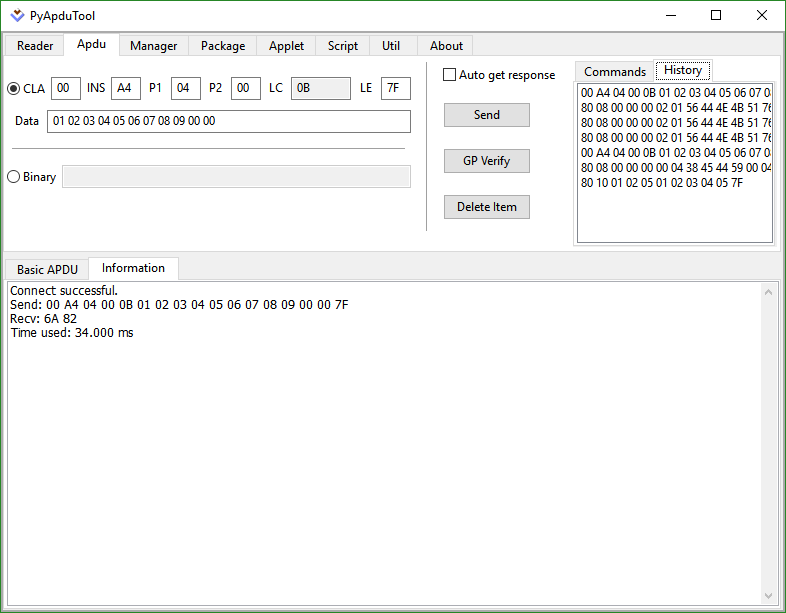
\includegraphics[width=0.95\textwidth]{images/pyapdutool.png}
\end{figure}

PyApduTool does not support extended APDU and this limits us to a high degree when testing our smart card application. Testing through PyApduTool does not test mobile device behavior such as: out of memory, too much traffic or NFC limitations. Another key point is that it is difficult to create test tools that works all smart cards as manufacturers make small adjustments in their version of Java Card. The results was that we often encountered weird errors with seemingly no clear cause. After the initial basic testing, PyApduTool became obsolete and we had to test via an Android application.

As a result we are very limited when it comes to testing the performance of the smart cards. The only way of measuring resource usage on the smart cards are with time stamps and by looking at the elapsed time do an evaluation on the performance. This makes it difficult to identify bottlenecks on the smart cards.

\subsection{Android application}
The second part of the framework is an Android library. The library will serve as an intermediate between the Android application and the smart card application.

\paragraph{Android version}\mbox{}\\
When we started working on the Android library, our mobile devices were running Android 4.4 (API level 19). By the end of this thesis Android 6.0 became more popular and we were able to migrate our framework to Android 6.0. The minimum SDK required for the library is API level 19 (Android 4.4) and the target SDK is API level 23 (Android 6.0). Google frequently provides data on what Android versions their user base uses. As of May 2, 2016, Android version 4.4 to 6.0 covered approximately 78\% of the users \cite{AndroidAPIDistributions}. Our opinion is that covering \~78\% of the user base is a realistic and sufficient goal.

\paragraph{IDE}\mbox{}\\
Android Studio \cite{androidIDE} is the official IDE for Android application development. Android Studio is based on IntelliJ IDEA \cite{intelliJIDEA} and provides many automated tools for building, deploying and publishing Android applications. Android Studio ships with Android Debug Bridge (ADB). ADB is an interface for communicating with virtual Android instances or physical Android devices. ADB gives developers the ability to log output from applications as well as monitor memory, GPU and CPU usage of the mobile device.

We utilize the log ability of ADB to great extent as it is more efficient in our case to look at byte values rather than constructing complex graphical user interface elements for our use cases. In essence, the log output from ADB is our graphical user interface when testing the various functions of the framework.

\paragraph{Test environment}\mbox{}\\
To test the application we will be using the built in ADB in Android studio as well as doing empirical tests on the Android device. Figure \ref{fig:ADBMemory} and \ref{fig:ADBCPU} shows runtime examples of the Android device. These monitor tools gives us a clear indication if we are doing an operation the Android device cannot handle or if we are trying to perform operations that are too resource intensive.

\begin{figure}[h!]
  \captionsetup{justification=centering,margin=1.5cm}
  \caption{Android Debug Bridge memory monitor connected to a running Android device.}
  \label{fig:ADBMemory}
  \centering
    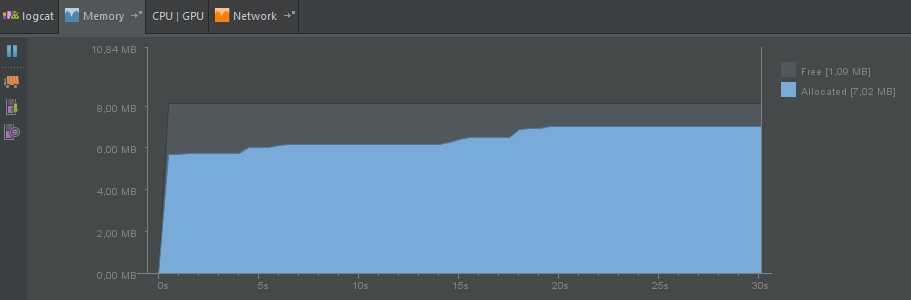
\includegraphics[width=0.95\textwidth]{images/ADBMemory.png}
\end{figure}

\begin{figure}[h!]
  \captionsetup{justification=centering,margin=1.5cm}
  \caption{Android Debug Bridge CPU monitor connected to a running Android device.}
  \label{fig:ADBCPU}
  \centering
    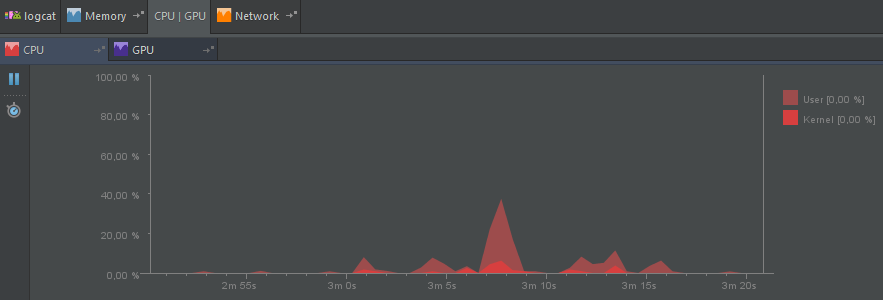
\includegraphics[width=0.95\textwidth]{images/ADBCPU.png}
\end{figure}

Even though ADB provides us with good resource usage tools we wish to perform more informal tests using timers to get a feel for how long an operation takes. We can use the built in Android class \texttt{System} and the method \texttt{nanoTime()} to get an accurate start and stop time for an operation and calculate elapsed time. This combined with visually inspecting the running application can help us get an indication of how responsive the application is when executing tasks.

\section{Development flow}
Recall the tools and technologies from the previous sections. Figure \ref{fig:devFlow} shows the development process. The process is linear from top to bottom, but it is important to note that we will need to develop for both the Android application and smart card applet in parallel. By parallel we mean that in order to test some new functionality we will need to implement functionality on both platforms.

The figure clearly shows that everything concerning the Android side of the framework is handled by Android Studio along with the Android SDK except for the Gemalto library for micro SD support. Google has put a lot of resources into streamlining the Android development process whereas we are dependent on independent or proprietary software for smart card applet development.

One important thing to note is that the figure shows that we cannot observe any test results of the smart card. Observation of the smart card's test results must be done via the Android application (refer to section \ref{sec:experience}).

\begin{figure}[h!]
  \caption{Development flow of the smart card framework}
  \label{fig:devFlow}
  \centering
    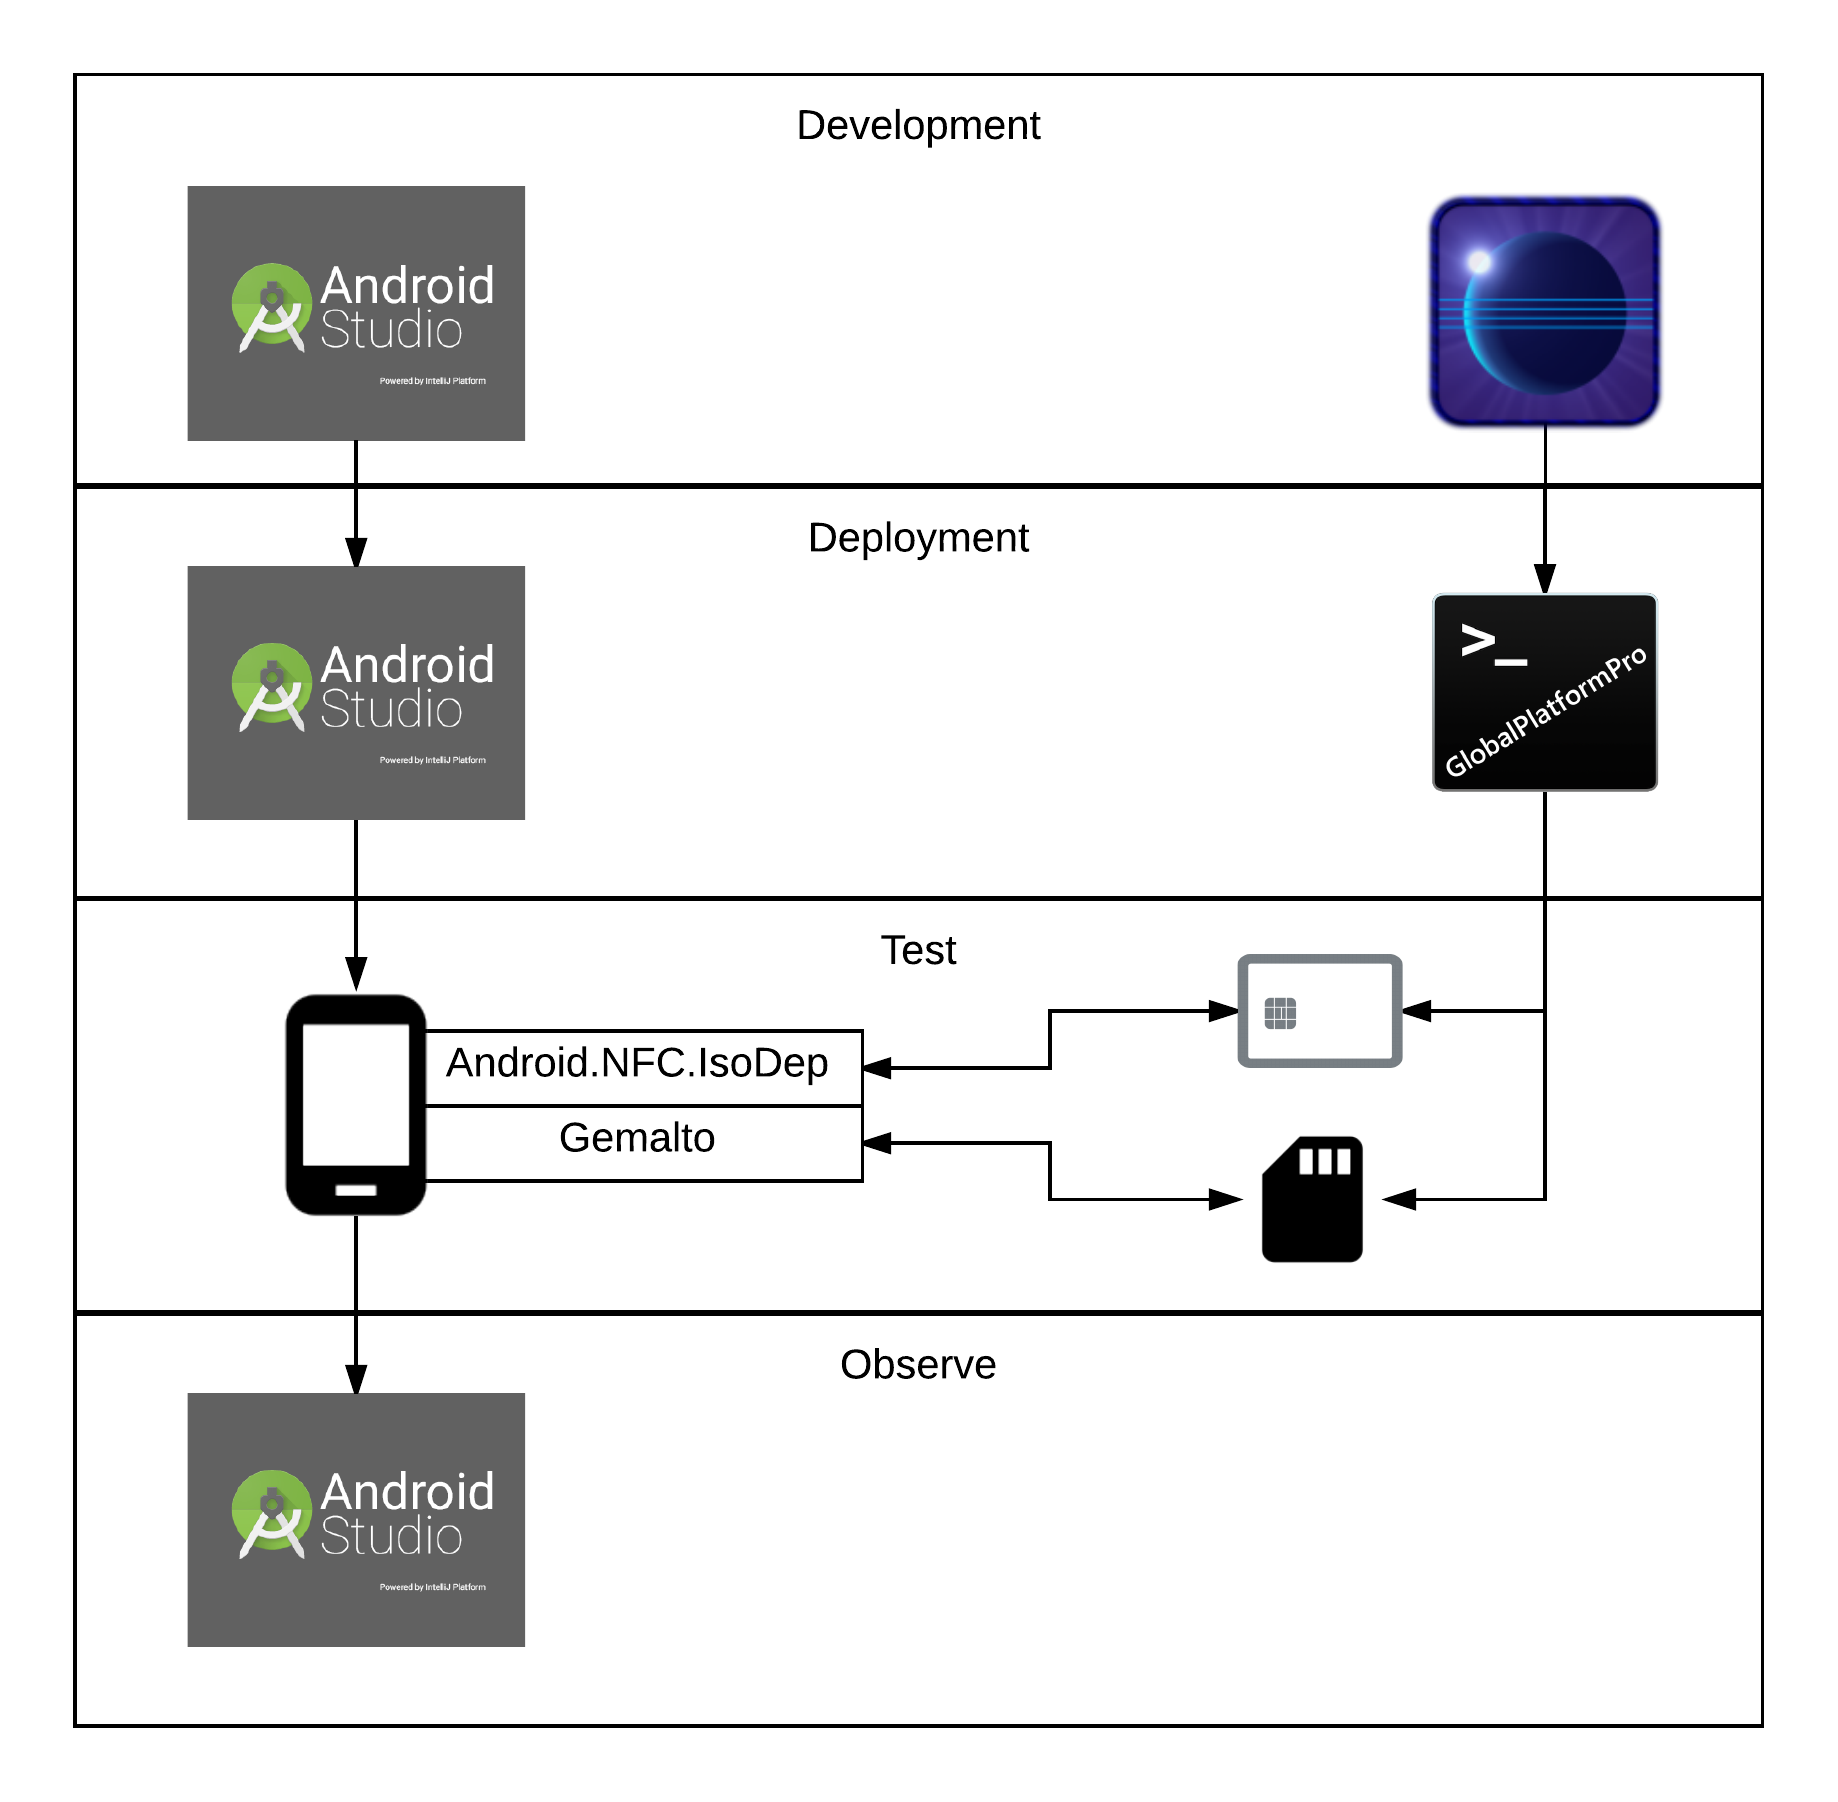
\includegraphics[width=0.95\textwidth]{images/devFlow.png}
\end{figure}
